\RequirePackage[l2tabu,orthodox]{nag}

% two-sided
\documentclass[headsepline,footsepline,footinclude=false,fontsize=11pt,paper=a4,listof=totoc,bibliography=totoc,BCOR=12mm,DIV=12]{scrbook} % two-sided
% \documentclass[headsepline,footsepline,footinclude=false,oneside,fontsize=11pt,paper=a4,listof=totoc,bibliography=totoc]{scrbook} % one-sided

\PassOptionsToPackage{table,svgnames,dvipsnames}{xcolor}

\usepackage[utf8]{inputenc}
\usepackage[T1]{fontenc}
\usepackage[sc]{mathpazo}
\usepackage[ngerman,american]{babel}
\usepackage[autostyle]{csquotes}
\usepackage[%
  backend=biber,
  url=false,
  sorting=ynt,
  style=numeric,
  maxnames=4,
  minnames=3,
  maxbibnames=99,
  giveninits,
  uniquename=init]{biblatex}
\usepackage{graphicx}
\usepackage{scrhack} % necessary for listings package
\usepackage{listings}
\usepackage{lstautogobble}
\usepackage{tikz}
\usepackage{pgfplots}
\usepackage{pgfplotstable}
\usepackage{booktabs}
\usepackage[final]{microtype}
\usepackage{caption}
\usepackage[hidelinks]{hyperref} % hidelinks removes colored boxes around references and links
\usepackage{amsmath}
\usepackage{mathtools}
\usepackage{amsthm,thmtools}
\usepackage[nottoc]{tocbibind}
\usepackage[ruled]{algorithm2e}
\usepackage{enumerate}
\usepackage{tabularx}
% \usepackage{ltablex}
\usepackage{imakeidx}

\DeclareMathOperator*{\argmax}{arg\,max}
\DeclareMathOperator*{\argmin}{arg\,min}

\makeindex[intoc]

\DeclarePairedDelimiter{\norm}{\lVert}{\rVert}

\declaretheorem[name=Theorem]{theorem}
\declaretheorem[name=Lemma,sibling=theorem]{lemma}
\declaretheorem[name=Definition,sibling=theorem]{definition}
\declaretheorem[name=Problem,sibling=theorem]{problem}
\makeatletter
\def\ll@problem{
  \protect\numberline{\theproblem}\thmt@shortoptarg
}
\makeatother

\renewcommand{\thealgocf}{\arabic{theorem}}

\bibliography{sources}

\setkomafont{disposition}{\normalfont\bfseries} % use serif font for headings
\linespread{1.05} % adjust line spread for mathpazo font

% Add table of contents to PDF bookmarks
\BeforeTOCHead[toc]{{\cleardoublepage\pdfbookmark[0]{\contentsname}{toc}}}

% Define TUM corporate design colors
% Taken from http://portal.mytum.de/corporatedesign/index_print/vorlagen/index_farben
\definecolor{TUMBlue}{HTML}{0065BD}
\definecolor{TUMSecondaryBlue}{HTML}{005293}
\definecolor{TUMSecondaryBlue2}{HTML}{003359}
\definecolor{TUMBlack}{HTML}{000000}
\definecolor{TUMWhite}{HTML}{FFFFFF}
\definecolor{TUMDarkGray}{HTML}{333333}
\definecolor{TUMGray}{HTML}{808080}
\definecolor{TUMLightGray}{HTML}{CCCCC6}
\definecolor{TUMAccentGray}{HTML}{DAD7CB}
\definecolor{TUMAccentOrange}{HTML}{E37222}
\definecolor{TUMAccentGreen}{HTML}{A2AD00}
\definecolor{TUMAccentLightBlue}{HTML}{98C6EA}
\definecolor{TUMAccentBlue}{HTML}{64A0C8}

% Settings for pgfplots
\pgfplotsset{compat=newest}
\pgfplotsset{
  % For available color names, see http://www.latextemplates.com/svgnames-colors
  cycle list={TUMBlue\\TUMAccentOrange\\TUMAccentGreen\\TUMSecondaryBlue2\\TUMDarkGray\\},
}

% Settings for lstlistings
\lstset{%
  basicstyle=\ttfamily,
  columns=fullflexible,
  autogobble,
  keywordstyle=\bfseries\color{TUMBlue},
  stringstyle=\color{TUMAccentGreen}
}

% Colors
\def\b{\textcolor{blue}}
\def\r{\textcolor{red}}

% Ternary operator
\newcommand{\ternary}[3]{\textbf{if}\ #1\ \textbf{then}\ #2\ \textbf{else}\ #3}


% thesis information
\newcommand*{\getUniversity}{Technical University of Munich}
\newcommand*{\getFaculty}{Department of Informatics}
\newcommand*{\getTitle}{Implementation of Algorithms for Right-Sizing Data Centers}
\newcommand*{\getTitleGer}{Implementierung von Algorithmen für die Größenanpassung von Rechenzentren}
\newcommand*{\getAuthor}{Jonas Hübotter}
\newcommand*{\getDoctype}{Bachelor's Thesis in Informatics}
\newcommand*{\getSupervisor}{Prof. Dr. Susanne Albers}
\newcommand*{\getAdvisor}{Jens Quedenfeld}
\newcommand*{\getSubmissionDate}{July 31, 2021}
\newcommand*{\getSubmissionLocation}{Munich}

\makenoidxglossaries

% basic notation
\glsxtrnewsymbol[description={\ensuremath{\{1, \dots, n\}}, for \ensuremath{n \in \mathbb{N}}}]{range}{\ensuremath{[n]}}
\glsadd{range}
\glsxtrnewsymbol[description={\ensuremath{\{0\} \cup [n]}, for \ensuremath{n \in \mathbb{N}}}]{0range}{\ensuremath{[n]_0}}
\glsadd{0range}
\glsxtrnewsymbol[description={\ensuremath{\max\{0, x\}}, for \ensuremath{x \in \mathbb{R}}}]{positive}{\ensuremath{(x)^+}}
\glsadd{positive}
\glsxtrnewsymbol[description={smallest entry of the vector \ensuremath{x}}]{vec_min}{\ensuremath{x_{min}}}
\glsadd{vec_min}
\glsxtrnewsymbol[description={largest entry of the vector \ensuremath{x}}]{vec_max}{\ensuremath{x_{max}}}
\glsadd{vec_max}

% symbols


\begin{document}

% Set page numbering to avoid "destination with the same identifier has been already used" warning for cover page.
% (see https://en.wikibooks.org/wiki/LaTeX/Hyperlinks#Problems_with_Links_and_Pages).
\pagenumbering{alph}
\begin{titlepage}
  % HACK for two-sided documents: ignore binding correction for cover page.
  % Adapted from Markus Kohm's KOMA-Script titlepage=firstiscover handling.
  % See http://mirrors.ctan.org/macros/latex/contrib/koma-script/scrkernel-title.dtx,
  % \maketitle macro.
  \oddsidemargin=\evensidemargin\relax
  \textwidth=\dimexpr\paperwidth-2\evensidemargin-2in\relax
  \hsize=\textwidth\relax

  \centering
  \null
  \vspace{18mm}
  \IfFileExists{thesis/logos/tum.pdf}{%
    
\includegraphics[height=20mm]{thesis/logos/tum.pdf}
  }{%
    \vspace*{20mm}
  }

  \vspace{10mm}
  {\huge\MakeUppercase{\getFaculty{}}}\\

  \vspace{5mm}
  {\large\MakeUppercase{\getUniversity{}}}\\

  \vspace{20mm}
  {\Large \getDoctype{}}

  \vspace{15mm}
  {\huge\bfseries \getTitle{}}

  \vspace{15mm}
  {\LARGE \getAuthor{}}

  \IfFileExists{thesis/logos/faculty.pdf}{%
    \vfill{}
    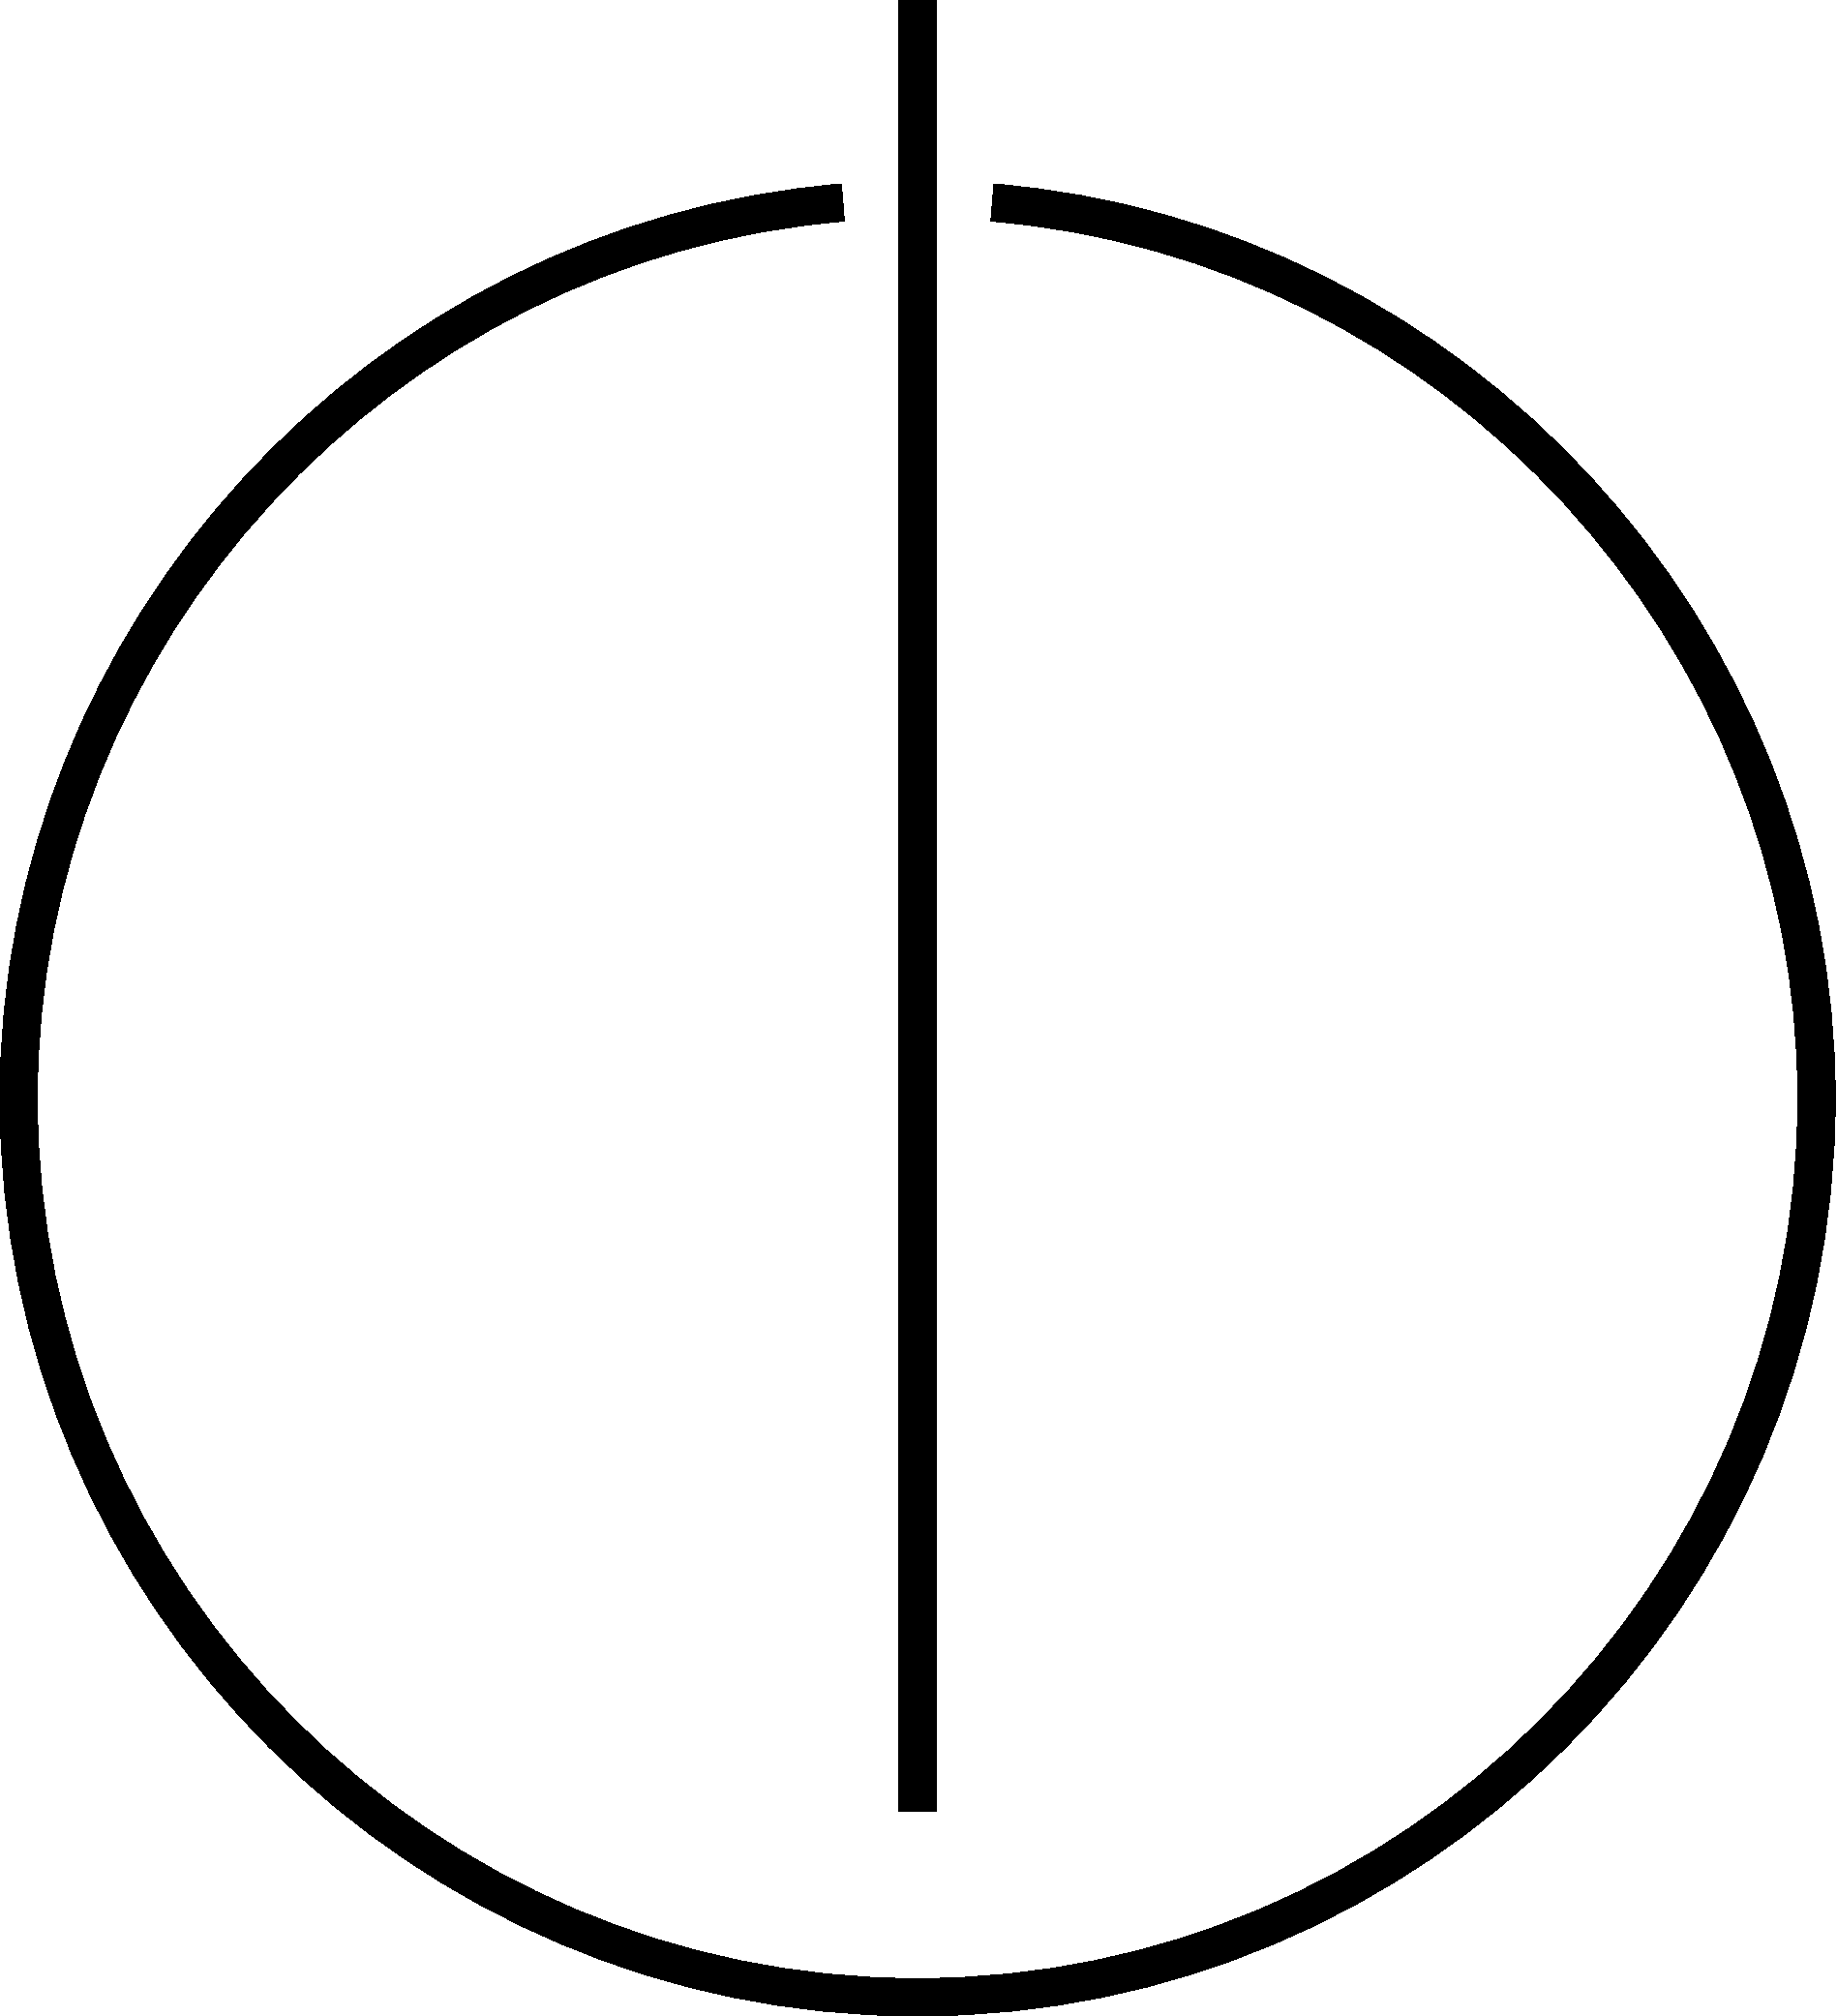
\includegraphics[height=20mm]{thesis/logos/faculty.pdf}
  }{}
\end{titlepage}

\frontmatter{}

\begin{titlepage}
  \centering

  \IfFileExists{thesis/logos/tum.pdf}{%
    
\includegraphics[height=20mm]{thesis/logos/tum.pdf}
  }{%
    \vspace*{20mm}
  }

  \vspace{10mm}
  {\huge\MakeUppercase{\getFaculty{}}}\\

  \vspace{5mm}
  {\large\MakeUppercase{\getUniversity{}}}\\

  \vspace{20mm}
  {\Large \getDoctype{}}

  \vspace{15mm}
  {\huge\bfseries \getTitle{}}

  \vspace{10mm}
  {\huge\bfseries \foreignlanguage{ngerman}{\getTitleGer{}}}

  \vspace{15mm}
  \begin{tabular}{l l}
    Author:          & \getAuthor{} \\
    Supervisor:      & \getSupervisor{} \\
    Advisor:         & \getAdvisor{} \\
    Submission Date: & \getSubmissionDate{} \\
  \end{tabular}

  \vspace{6mm}
  \IfFileExists{thesis/logos/faculty.pdf}{%
    \vfill{}
    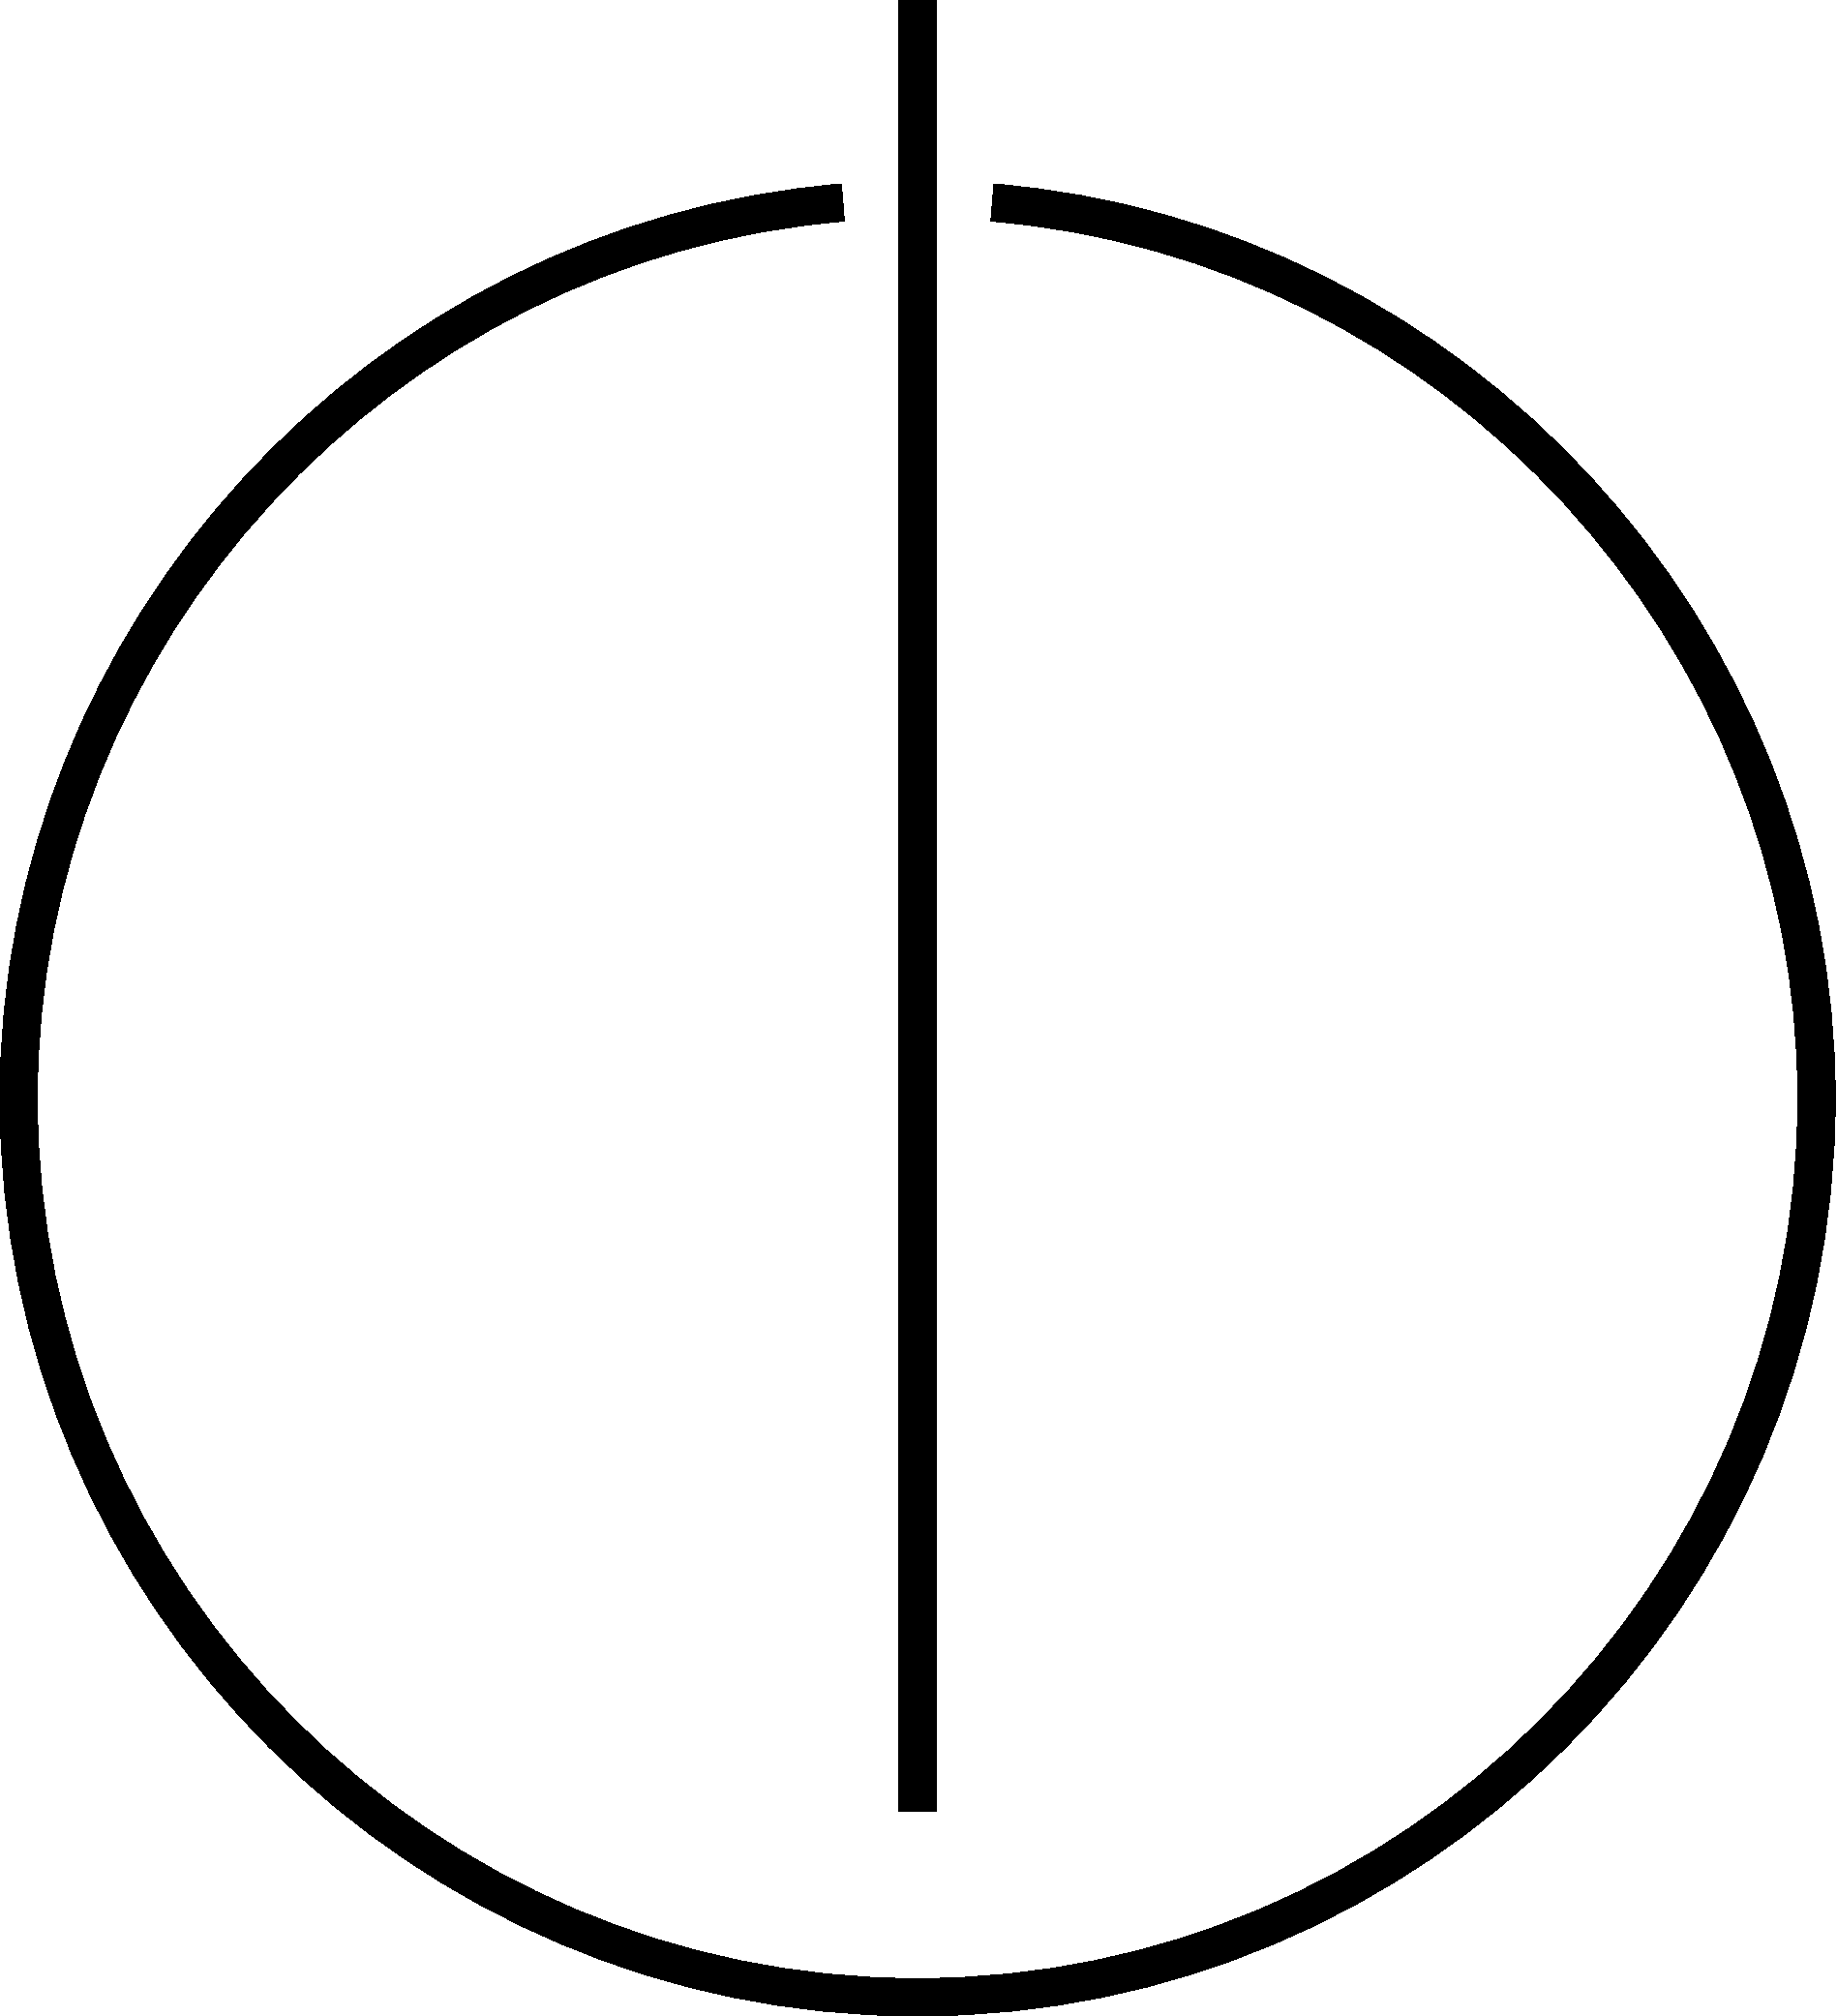
\includegraphics[height=20mm]{thesis/logos/faculty.pdf}
  }{}
\end{titlepage}
\cleardoublepage{}

\thispagestyle{empty}
\vspace*{0.8\textheight}
\noindent
I confirm that this bachelor's thesis is my own work and I have documented all sources and material used.

\vspace{15mm}
\noindent
\getSubmissionLocation{}, \getSubmissionDate{} \hspace{50mm} \getAuthor{}

\cleardoublepage{}

\addcontentsline{toc}{chapter}{Acknowledgments}
\thispagestyle{empty}

\vspace*{20mm}

\begin{center}
{\usekomafont{section} Acknowledgments}
\end{center}

\vspace{10mm}

%TODO: Acknowledgments

\cleardoublepage{}

\chapter{\abstractname}

The energy consumption of data centers assumes a significant fraction of the worlds overall energy consumption. Most data centers are statically provisioned leading to a very low average utilization of servers. In this work we survey uni-dimensional and high-dimensional approaches for dynamically powering-up and powering-down servers to reduce the energy footprint of data centers while ensuring that incoming jobs are processed in-time. We implement algorithms for smoothed online convex optimization and variations thereof where in each round the agent receives a convex cost function. The agent seeks to minimize cost based on an exploration-exploitation trade-off using an additional switching cost which is associated with changing decisions in-between rounds. We implement the algorithms in their most general form, inviting future research on their performance in other application areas. We evaluate the algorithms for the application of right-sizing data centers using traces from Facebook, Microsoft, Alibaba, and Los Alamos National Lab. Our experiments show that the the online algorithms perform close to the dynamic offline optimum in practice and promise a significant cost reduction when compared to the static offline optimum. We discuss how features of the data center model and trace impact the performance. Finally, we investigate the practical use of predictions to achieve further cost reductions.

\microtypesetup{protrusion=false}
\tableofcontents{}
\microtypesetup{protrusion=true}

\mainmatter{}

% !TeX root = ../main.tex
% Add the above to each chapter to make compiling the PDF easier in some editors.

\chapter{Introduction}\label{chapter:introduction}

\section{Section}
Citation test~\parencite{latex}.

\subsection{Subsection}

See~\autoref{tab:sample}, \autoref{fig:sample-drawing}, \autoref{fig:sample-plot}, \autoref{fig:sample-listing}.

\begin{table}[htpb]
  \caption[Example table]{An example for a simple table.}\label{tab:sample}
  \centering
  \begin{tabular}{l l l l}
    \toprule
      A & B & C & D \\
    \midrule
      1 & 2 & 1 & 2 \\
      2 & 3 & 2 & 3 \\
    \bottomrule
  \end{tabular}
\end{table}

\begin{figure}[htpb]
  \centering
  % This should probably go into a file in figures/
  \begin{tikzpicture}[node distance=3cm]
    \node (R0) {$R_1$};
    \node (R1) [right of=R0] {$R_2$};
    \node (R2) [below of=R1] {$R_4$};
    \node (R3) [below of=R0] {$R_3$};
    \node (R4) [right of=R1] {$R_5$};

    \path[every node]
      (R0) edge (R1)
      (R0) edge (R3)
      (R3) edge (R2)
      (R2) edge (R1)
      (R1) edge (R4);
  \end{tikzpicture}
  \caption[Example drawing]{An example for a simple drawing.}\label{fig:sample-drawing}
\end{figure}

\begin{figure}[htpb]
  \centering

  \pgfplotstableset{col sep=&, row sep=\\}
  % This should probably go into a file in data/
  \pgfplotstableread{
    a & b    \\
    1 & 1000 \\
    2 & 1500 \\
    3 & 1600 \\
  }\exampleA
  \pgfplotstableread{
    a & b    \\
    1 & 1200 \\
    2 & 800 \\
    3 & 1400 \\
  }\exampleB
  % This should probably go into a file in figures/
  \begin{tikzpicture}
    \begin{axis}[
        ymin=0,
        legend style={legend pos=south east},
        grid,
        thick,
        ylabel=Y,
        xlabel=X
      ]
      \addplot table[x=a, y=b]{\exampleA};
      \addlegendentry{Example A};
      \addplot table[x=a, y=b]{\exampleB};
      \addlegendentry{Example B};
    \end{axis}
  \end{tikzpicture}
  \caption[Example plot]{An example for a simple plot.}\label{fig:sample-plot}
\end{figure}

\begin{figure}[htpb]
  \centering
  \begin{tabular}{c}
  \begin{lstlisting}[language=SQL]
    SELECT * FROM tbl WHERE tbl.str = "str"
  \end{lstlisting}
  \end{tabular}
  \caption[Example listing]{An example for a source code listing.}\label{fig:sample-listing}
\end{figure}

% !TeX root = ../main.tex
% Add the above to each chapter to make compiling the PDF easier in some editors.

\chapter{Theory}\label{chapter:theory}

\section{Problems}

\subsection{Smoothed Convex Optimization}

\begin{problem}[Smoothed Convex Optimization (SCO)]
Given a time horizon $T \in \mathbb{N}$, a convex decision space $\mathcal{X} \subset \mathbb{R}^d$, a norm $\norm{\cdot}$ on $\mathbb{R}^d$, and a sequence of non-negative convex functions $f_t$ for $t \in [T]$ with $f_t(x) = \infty$ for all $x \not\in \mathcal{X}$, find $x \in \mathcal{X}$ minimizing \begin{align*}
    c(x) = \sum_{t=1}^T f_t(x_t) + \norm{x_t - x_{t-1}}
\end{align*}
where $x_0 = 0$.
\end{problem}

In many practical applications of Smoothed Convex Optimization, we seek to find integral solutions minimizing hitting and switching costs. This is especially true within the context of resource allocation, for example for right-sizing data centers, where our resources are discrete. This observation motivates the definition of the following variant of SCO.

\begin{problem}[Integral Smoothed Convex Optimization (Int-SCO)]
We define Integral Smoothed Convex Optimization analogously to SCO with the added restriction that the points $x$ in $d$-dimensional space must be discrete, that is $\mathcal{X} \subset \mathbb{Z}^d$.
\end{problem}

\subsubsection{Complexity of the Offline Problem}

We now want to examine the complexity of Int-SCO in the offline case. That is, we know all arriving convex cost functions $f_t$ in advance. We prove Int-SCO NP-hard for varying $d$ by giving a polynomial-time reduction from the Knapsack problem. In \autoref{section:theory:simplified_smoothed_convex_optimization} we first extend this proof of NP-hardness to the Integral Simplified Smoothed Convex Optimization problem which restricts the decision space and switching cost. Then, in \autoref{section:theory:smoothed_balanced_load_optimization}, we extend the proof to the Integral Smoothed Balanced-Load Optimization problem which further restricts the structure of the cost functions.

Given a set of items with an associated value and weight and an upper bound to the total weight, Knapsack is the problem of determining the number of copies of each item that maximizes the total value and conforms to the given upper bound on total weight. Formally we define Knapsack as follows.

\begin{problem}[Knapsack (KP)]
Given a number of items $n \in \mathbb{N}$, a value of each item $v \in \mathbb{N}^n$, a weight of each item $w \in \mathbb{N}^n$, and an upper bound to the total weight $W \in \mathbb{N}$, find $x \in \{0,1\}^n$ satisfying $\sum_{i = 1}^n w_i x_i \leq W$ and maximizing $\sum_{i=1}^n v_i x_i$.
is maximized.
\end{problem}

This variant of Knapsack is commonly called \textit{0-1 Knapsack} and restricts the number of copies of each item to be either 0 or 1. It is, however, easy to see that our proof can easily be generalized to a setting where we allow $x_i \in [m_i]_0$ for $m \in \mathbb{N}^n$. TODO et al. show that the Knapsack decision problem is NP-complete and that the Knapsack optimization problem is NP-hard.

Before reducing to Int-SCO, we reduce Knapsack to a related problem called Minimum Knapsack.

\begin{problem}[Minimum Knapsack (Min-KP)]
Given a number of items $n \in \mathbb{N}$, a cost of each item $c \in \mathbb{N}^n$, a utility of each item $u \in \mathbb{N}^n$, and a lower bound to the total utility $U \in \mathbb{N}$, find $x \in \{0,1\}^n$ satisfying $\sum_{i = 1}^n u_i x_i \geq U$ and minimizing $\sum_{i=1}^n c_i x_i$.
\end{problem}

\begin{lemma}
Min-KP is NP-hard.
\end{lemma}

\begin{proof}
We prove the lemma by giving a reduction from KP.

Let $\mathcal{I}_1 = (n, v, w, W)$ be an instance of KP. Let $\mathcal{I}_2(U) = (n, c, u, U)$ be an instance of Min-KP with $c = w$, and $u = v$. Hence, $\mathcal{I}_2(U)$ minimizes the total weight $\sum_{i=1}^n w_i x_i$ such that $\sum_{i=1}^n v_i x_i \geq U$.

By finding solutions to $\mathcal{I}_2(U)$ repeatedly for varying $U$, we determine the maximal $U$ such that $\sum_{i=1}^n w_i x_i \leq W$. Let $v_{max} = \max\{v_i \mid i \in [n]\}$ be the maximal value of any item. We observe that $U$ is upper bounded by $n \cdot v_{max}$. If $U$ were greater than $n \cdot v_{max}$ we would have $\sum_{i=1}^n v_{max} x_i \geq \sum_{i=1}^n v_i x_i > n \cdot v_{max}$ which contradicts $x \in \{0,1\}^n$. Hence, we can use binary search to find $U$ in $\mathcal{O}(\log n + \log v_{max})$ iterations. The other direction works analogously.

We have seen a total, polynomial-time reduction from KP to Min-KP. Hence, Min-KP is NP-hard.
\end{proof}

Next we prove our main reduction from Min-KP to Int-SCO. To motivate this reduction, we first prove that the following (convex) integer optimization is in fact equivalent to Min-KP.

\begin{lemma}
\label{lemma:integer_minimization}
Let $\mathcal{I} = (n, c, u, U)$ be an instance of Min-KP. $x$ is the solution to $\mathcal{I}$ if and only if $x$ minimizes \begin{align*}
    c'(x) = \sum_{i=1}^n c_i x_i + M(U - \sum_{i=1}^n u_i x_i)^+
\end{align*} subject to $x \in \{0,1\}^n$ for some $M > \frac{c_{max}}{u_{min}}$.
\end{lemma}

\begin{proof}
Suppose $x$ minimizes $c'(x)$. Now suppose $(U - \sum_{i=1}^n u_i x_i)^+ > 0$. Then, $(U - \sum_{i=1}^n u_i x_i)^+ \geq u_{min}$. Therefore, $c'(x) > \sum_{i=1}^n c_i x_i + c_{max}$. We observe that $x$ is not optimal as either $c'(x)$ could be minimized further by increasing $x$ such that $(U - \sum_{i=1}^n u_i x_i)^+ = 0$ since $\sum_{i=1}^n c_i x_i \leq c_{max}$ holds for all $x$. Alternatively, $x$ already equals 1 in each dimension in which case $\sum_{i=1}^n u_i < U$, indicating that $\mathcal{I}$ has no solution.

By leading our previous assumption to a contradiction, we conclude $(U - \sum_{i=1}^n u_i x_i)^+ = 0$ and therefore $U \leq \sum_{i=1}^n u_i x_i$. Further, $c'(x)$ minimizes $\sum_{i=1}^n c_i x_i$ for all remaining candidates for $x$. Hence, $x$ is the solution of $\mathcal{I}$.

On the other hand, suppose that $x$ is the solution to $\mathcal{I}$. Then $(U - \sum_{i=1}^n u_i x_i)^+ = 0$ and $\sum_{i=1}^n c_i x_i$ is minimized. Hence, $x$ minimizes $c'(x)$.
\end{proof}

For our construction we need that $c$ is convex.

\begin{lemma}
\label{lemma:integer_minimization_convexity}
$c'(\cdot)$ is convex.
\end{lemma}

\begin{proof}
It is easy to see that $c$ is continuous. Therefore, to show the convexity of $c$ it suffices to prove $c'(\frac{x+y}{2}) \leq \frac{c'(x)+c'(y)}{2}$ for all $x, y \in \mathbb{R}^n$.

To simplify the notation let $c'(x) = \sum_{i=1}^n c_i x_i$ and let $U(x) = \sum_{i=1}^n u_i x_i$. To further simplify the notation we define $\frac{x+y}{2}$ to be applied component-wise to elements $i \in [n]$ of $x$ and $y$. We then obtain \small{
\begin{align*}
         &c'(\frac{x+y}{2}) \leq \frac{c'(x)+c'(y)}{2} \\
    \iff &C(\frac{x+y}{2}) + M(U - U(\frac{x+y}{2}))^+ \leq \frac{C(x) + M(U - U(x))^+ + C(y) + M(U - U(y))^+}{2} \\
    \iff &C(x) + C(y) + 2M(U - U(\frac{x+y}{2}))^+ \leq C(x) + M(U - U(x))^+ + C(y) + M(U - U(y))^+ \\
    \iff &2(U - U(\frac{x+y}{2}))^+ \leq (U - U(x))^+ + (U - U(y))^+.
\end{align*}
}\normalsize

We immediately get the convexity of $U(\cdot)$ by the following equivalence. \begin{align*}
    U(\frac{x+y}{2}) &= \sum_{i=1}^n u_i \frac{x_i + y_i}{2} \\
                     &= \frac{\sum_{i=1}^n u_i x_i + \sum_{i=1}^n u_i y_i}{2} \\
                     &= \frac{U(x) + U(y)}{2}.
\end{align*}

Now, we consider three cases separately.

\begin{enumerate}
    \item If $U(x) > U$ and $U(y) > U$, then $U(\frac{x+y}{2}) > U$. Hence \begin{align*}
        2(U - U(\frac{x+y}{2}))^+ = 0 = (U - U(x))^+ + (U - U(y))^+.
    \end{align*}
    \item If $U(x) \leq U$ and $U(y) \leq U$, then $U(\frac{x+y}{2}) \leq U$. Hence \begin{align*}
        2(U - U(\frac{x+y}{2}))^+ &= 2U - 2U(\frac{x+y}{2}) \\
                                  &= 2U - U(x) + U(y) \\
                                  &= (U - U(x))^+ + (U - U(y))^+.
    \end{align*}
    \item For the only remaining case we assume w.l.o.g. that $U(x) \leq U$ and $U(y) > U$. If $U - U(x) < U(y) - U$, then $U(\frac{x+y}{2}) > U$ and we follow the first case. If, on the other hand, $U - U(x) \geq U(y) - U$, then $U(\frac{x+y}{2}) \leq U$ and we follow the second case.\qedhere
\end{enumerate}
\end{proof}

We now have everything in place to prove our main result of this section.

\begin{theorem}
Int-SCO is NP-hard.
\end{theorem}

\begin{proof}
We now give our reduction from Min-KP to Int-SCO.

Let $\mathcal{I}_1 = (n, c, u, U)$ be an instance of Min-KP. We define $\mathcal{I}_2 = (T, \mathcal{X}, \norm{\cdot}, f)$ as an instance of Int-SCO with $T = 1$, $\mathcal{X} = \{0,1\}^n$, $\norm{\cdot} = 0$, and $f_1(x) = c'(x)$. We further set $d = n$. By \autoref{lemma:integer_minimization_convexity}, $\mathcal{I}_2$ is a valid instance of Int-SCO.

The correctness of our construction follows from \autoref{lemma:integer_minimization}.

\begin{align*}
         &x \text{ is a solution to } \mathcal{I}_2 \\
    \iff &x \text{ minimizes } \sum_{t=1}^T f_t(x_t) + \norm{x_t - x_{t-1}} \text{ such that } x_t \in \mathcal{X}. \\
    \iff &x \text{ minimizes } c'(x_1) \text{ such that } x_1 \in \{0,1\}^n. \\
    \iff &x_1 \text{ is a solution to } \mathcal{I}_1.
\end{align*}

Our construction is total and polynomial in the size of $\mathcal{I}_1$. Hence, Int-SCO is NP-hard.
\end{proof}

We observe that the above reduction can be extended to Knapsack with arbitrary bounds $m_i$ by setting $\mathcal{X}$ of $\mathcal{I}_2$ to $[m_1]_0 \times \dots \times [m_n]_0$.

\subsection{Simplified Smoothed Convex Optimization}
\label{section:theory:simplified_smoothed_convex_optimization}

In many applications, for example for right-sizing data centers, it suffices to restrict $\mathcal{X}$ to $\mathcal{X} = [m_0]_0 \times \dots \times [m_d]_0$ for some $m \in \mathbb{N}^d$ and the switching cost $\norm{x}$ to $\sum_{k=1}^d \beta_k x_k^+$ where $\beta$ is constant for each dimension. To that end, we first define a restricted variant of (fractional) SCO which we term \textit{Simplified Smoothed Convex Optimization}.

\begin{problem}[Simplified Smoothed Convex Optimization (SSCO)]
Given a time horizon $T \in \mathbb{N}$, upper bounds $m \in \mathbb{N}^d$, switching costs $\beta \in \mathbb{R}_{>0}^d$, and a sequence of non-negative convex functions $f_t$ for $t \in [T]$, find $x \in \mathbb{R}_{\geq 0, \leq m_0} \times \dots \times \mathbb{R}_{\geq 0, \leq m_d}$ minimizing \begin{align*}
    c(x) = \sum_{t=1}^T f_t(x_t) + \sum_{k=1}^d \beta_k (x_{t,k} - x_{t-1,k})^+
\end{align*}
where $x_0 = 0$.
\end{problem}

We observe that $c(\cdot)$ pays the switching cost whenever $x$ increases. Decreasing $x$ does not increase the paid switching cost. This observation indicates that the following cost function $d(\cdot)$ is equivalent to $c(\cdot)$.

\begin{definition}[Inverted Simplified Smoothed Convex Optimization]
\begin{align*}
    d(x) = \sum_{t=1}^T f_t(x_t) + \sum_{k=1}^d \beta_k (x_{t,k} - x_{t+1,k})^+.
\end{align*}
Instead of $x_0 = 0$ we require $x_{T+1} = 0$.
\end{definition}

With the same motivation we used for the restriction of SCO to Int-SCO, we now restrict SSCO to an integral variant.

\begin{problem}[Integral Simplified Smoothed Convex Optimization (Int-SSCO)]
We define Integral Simplified Smoothed Convex Optimization analogously to SSCO with the added restriction that the points $x$ in $d$-dimensional space must be discrete, that is $x \in [m_0]_0 \times \dots \times [m_d]_0$.
\end{problem}

\subsubsection{Complexity of the Offline Problem}

We next extend our proof of NP-hardness of Int-SCO for varying $d$ to Int-SSCO. We cannot reuse our original proof as the switching cost of SSCO is required to be positive.

\subsection{Smoothed Balanced-Load Optimization}
\label{section:theory:smoothed_balanced_load_optimization}

\subsection{Smoothed Load Optimization}

\subsubsection{Complexity of the Offline Problem}

\section{Algorithm Analysis}

\subsection{Approximations}

\subsection{Regret}

\subsection{Competitiveness}

% !TeX root = ../main.tex
% Add the above to each chapter to make compiling the PDF easier in some editors.

\chapter{Application: Right-Sizing Data Centers}\label{chapter:application_data_centers}

\section{Server Infrastructures}

\section{Modeling Cost}

\subsection{Optimal Load Balancing}

\section{Modeling Time}

\section{Using Online Algorithms in Practice}

% !TeX root = ../main.tex
% Add the above to each chapter to make compiling the PDF easier in some editors.

\chapter{Application: Horizontal Container Scaling}\label{chapter:application_container_scaling}

% !TeX root = ../main.tex
% Add the above to each chapter to make compiling the PDF easier in some editors.

\chapter{Offline Algorithms}\label{chapter:algorithms}

\section{Uni-Dimensional}

\subsection{Capacity Provisioning}

\subsubsection{Backward-Recurrent}

\subsubsection{Forward-Recurrent}

\subsection{Graph-Based Optimal Discrete Algorithm}

\subsection{[Graph-Based Linear-Time Discrete Approximation Algorithm]}

\section{Multi-Dimensional}

\subsection{[Optimal Continuous Algorithm]}

\subsection{Graph-Based Optimal Discrete Algorithm}

\subsection{Graph-Based Polynomial-Time Discrete Approximation Algorithm}

% !TeX root = ../main.tex
% Add the above to each chapter to make compiling the PDF easier in some editors.

\chapter{Online Algorithms}\label{chapter:algorithms}

\section{Uni-Dimensional}

\subsection{Lazy Capacity Provisioning}

\subsubsection{Fractional Algorithm}

\subsubsection{Integral Algorithm}

\subsection{Memoryless Algorithm}

\subsection{Probabilistic Algorithm}

\subsection{Randomized Integral Relaxation}

\section{Multi-Dimensional}

\subsection{Lazy Budgeting}

\subsubsection{Lazy Budgeting for Smoothed Load Optimization}

\subsubsection{Randomized Lazy Budgeting for Smoothed Load Optimization}

\subsubsection{Lazy Budgeting for Smoothed Balanced-Load Optimization}

\section{Predicting}

\subsection{Prediction Window}

\subsubsection{Lazy Capacity Provisioning with Prediction Window}

% !TeX root = ../main.tex
% Add the above to each chapter to make compiling the PDF easier in some editors.

\chapter{Conclusion}\label{chapter:conclusion}

\section{Future Work}

% TODO: add more chapters here

% Examples
Citation test~\parencite{latex}.
Reference symbols: $\gls{x}$

\begin{figure}[htb]
    \centering
    Test
    \caption{Caption}
    \label{fig:my_label}
\end{figure}

\begin{algorithm}[H]
    \caption{Algorithm}
    \SetKwInOut{Input}{Input}
    \Input{something}
    step 1\;
    step 2\;
\end{algorithm}

\begin{definition}[Test]
...
\end{definition}

\begin{theorem}
...
\end{theorem}

\begin{problem}[Test]
...
\end{problem}

\appendix{}

\microtypesetup{protrusion=false}

\listoftheorems[ignoreall,show=problem,title={List of Problems}]{}

\listofalgorithms{}
\addcontentsline{toc}{chapter}{List of Algorithms}

% \listoffigures{}

\printnoidxglossary[type=symbols,style=long,title={Notation}]

\microtypesetup{protrusion=true}

\printbibliography{}

\end{document}
